\part{Les données}
    \chapter{Le périmètre produit}
    \label{perimetre_produit}

    \section{Les produits non-alimentaires}
    \label{produits_nonal}
    Un petit apparté est nécessaire concernant les produits non-alimentaires.
    Si l'essentiel des produits commercialisés par les branches du groupe sont des produits alimentaires, comme évoqué précédemment une partie de l'activité commerciale se fait tout de même autour de produits non-alimentaires.
    Ces produits restent malgré tout destinés exclusivement aux professionnels des métiers de bouche, et il s'agit de consommables (par opposition à des articles d'électroménager, de la vaisselle non-jetable, \dots).

    On distingue en général deux catégories de produits non-alimentaires : 
    \begin{itemize}
        \item les produits dits \og d'hygiène \fg
        \item les produits dits \og de chimie \fg
    \end{itemize}

    Les produits de chimie regroupent les produits qui doivent faire l'objet d'une fiche de données de sécurté au sens du réglement Européen No 1907/2006 dit \og REACH \fg (Registration, Evaluation, Authorisation and Restriction of Chemicals) \cite{reach_text}.

    On appelle produits d'hygiène tous les autres produits non-alimentaires.
    L'appelation \og d'hygiène \fg est donc réductricte, dans la mesure où cette large famille regroupe les consommables de nettoyage (éponges, papiers absorbants, \dots) mais également tout type d'autres consommables (serviettes de tables, gobelets en plastiques, pics à brochettes, boîtes de produits à emporter, \dots).

    \emphbox{La commercialisation de produits non-alimentaires existe au sein du groupe, mais on se focalisera pour la suite sur les produits alimentaires qui reste le coeur de métier.}

        \section{Accessibilité de la donnée en fonction des branches}

        Comme vu à la section \mref{outils_infos}, les systèmes d'information associés à la gestion de l'information produit offrent des niveaux d'accès hétérogènes à la donnée produit.
        Le récapitulatif par branche est le suivant : 
        \begin{description}
            \item[\'{E}piSaveurs :] on peut simplement accéder à l'ensemble des données produit, structurées, non structurées (i.e. textes longs) et pièces jointes
            \item[PassionFroid :] on a uniquement la possibilité d'exporter manuellement les données structurées articles depuis le système de gestion SAP.
            Elles permettent de produire quelques analyses quantitatives.
            Il est difficile de faire des exports en masse de l'outil de gestion de l'information produit GIP (cf. section \mref{GIP}).
            \item[TerreAzur :] idem PassionFroid, si ce n'est qu'en plus le système GIP n'est pas utilisé au sein de cette branche.
            \item[Délice et Création :] le système d'information ne permet pas d'exporter les données et donc de produire des indicateurs détaillés. On peut toutefois avoir des informations quantitatives de la part des opérationnels.
            \item[Saveurs d'Antoine :] idem Délice et Création
            \item[Pomona Suisse :] la branche est en cours de structuration, et les référentiels articles ne sont pas partagés entre les succursales. Il n'est pas possible d'obtenir d'information quantitative sur ces données.
            \item[Pomona Iberia :] idem Pomona Suisse
        \end{description}

        Pour les analyses quantitatives, on pourra se baser sur des extractions uniquement pour les branches RHD (\'{E}piSaveurs, PassionFroid, TerreAzur).
        L'ensemble des analyses portant sur les branches RHD sont produites sur la base d'extractions de leur système de gestion SAP.

        \section{Analyses quantitatives}

        Les graphes de cette section ont été produits via le code présenté en annexe, au chapitre \mref{code:analyse_quantitative}.
        Les données pour les branches spécialistes (Délice et Création et Saveurs d'Antoine) sont issues d'informations fournies par le métier, hors système.
        Dans l'ensemble de cette section, on raisonnera à la maille \emph{article} (cf. la définition article vs. produits, présentée à la section \mref{produit_article}).

            \subsection{Comparatifs entre les branches}

                En termes de volumétrie article (cf. \reffig{fig:volumetrie_article}, c'est TerreAzur qui possède le référentiel le plus étendu (environ 62 000 articles de marchandises actifs).
                Cela s'explique par le fait que cette branche commercialise essentiellement des produits bruts, non-préemballés (ex : des cagettes de fruits ou de légumes).
                Or, ces produits ne sont pas clairement identifiés, par exemple par un GTIN.
                Au démarrage de SAP pour cette branche, afin de limiter la charge sur les gestionnaires de référentiels, le parti a été pris de créer en avance de phase l'ensemble des articles susceptibles d'être commercialisés.
                Cela s'est traduit par la création d'un grand nombre d'articles, du fait de l'application \og brutale \fg de la combinatoire des différents critères pouvant définir un produit.
                Un exemple (fictif) serait, sur les pommes : 
                \begin{itemize}
                    \item 8 variétés possibles (Gala, Golden, \dots)
                    \item 4 calibres possibles
                    \item 6 conditionnements possibles (plateau 6kg, plateau 4,5kg, \dots)
                    \item 2 catégories (I, II)
                    \item 8 origines (France, Espagne, \dots)
                \end{itemize}
                ce qui donne un total de 3072 articles uniquement sur cette gamme de produits.

                Viennent ensuite PassionFroid, et \'{E}piSaveurs, qui sont les autres \og grosses \fg branches historiques du Groupe.

                \begin{figure}[htbp]\CenterFloatBoxes
                    \begin{floatrow}
                    \ffigbox{%
                        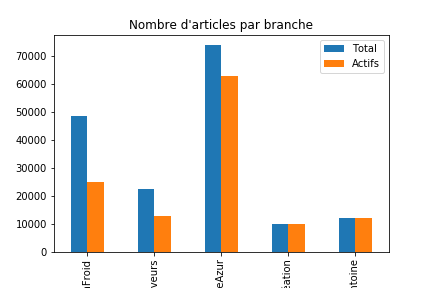
\includegraphics[width=200pt]{img/Articles par branche.png}%
                    }{%
                      \caption{Volumétrie article par branche}%
                      \label{fig:volumetrie_article}%
                    }
                    \capbtabbox[][][c]{%
                        \begin{tabular}{lccc}
\toprule
{} &  Total &  Actifs &  Marchandises \\
\textbf{Branche           } &        &         &               \\
\midrule
\textbf{PassionFroid      } &  48478 &   24898 &         24554 \\
\textbf{EpiSaveurs        } &  22498 &   12798 &         12241 \\
\textbf{TerreAzur         } &  73804 &   62789 &         62710 \\
\textbf{Délice et Création} &  10000 &       - &             - \\
\textbf{Saveurs d'Antoine } &  12000 &       - &             - \\
\bottomrule
\end{tabular}
%
                    }{%
                      \caption{Volumétrie article par branche}%
                    }
                    \end{floatrow}
                \end{figure}
                    
                Une analyse du recouvrement des référentiels montre que dans l'ensemble, les branches ne travaillent pas les mêmes articles (cf. \reffig{fig:venn_article}).
                PassionFroid commercialise certains produits des branches \'{E}piSaveurs et TerreAzur, mais cela s'explique par une petite entité luxembourgeoise qui travaille des produits de tout type de stockage.
                Une réserve toutefois par rapport à cette analyse de recouvrement produit : elle sous-estime vraisemblablement lesdits recouvrements, dans la mesure où la présence de doublons n'est pas prise en compte.

                \begin{figure}[htbp]
                    \begin{center}
                    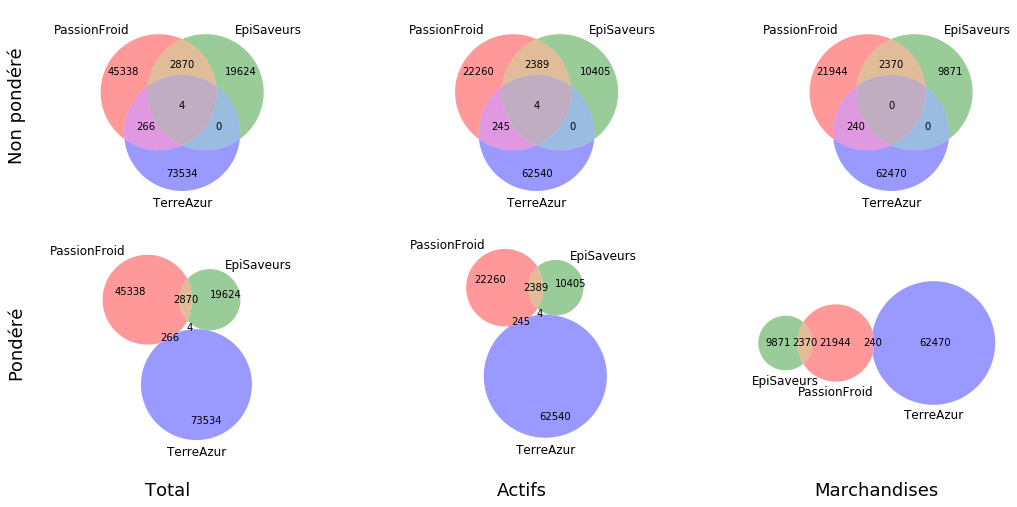
\includegraphics[width=\linewidth]{img/Diagrammes de Venn articles.png}
                    \end{center}
                    \caption{Recouvrements entre branches RHD}
                    \label{fig:venn_article}
                \end{figure}       

            \subsection{Les grands types de produits}

            Comme montré à la \reffig{fig:repart_art_categ}, on voit bien (en plus du fait que les articles étaient peu partagés entre les branches) que : 
            \begin{itemize}
                \item les deux types d'articles (négoce et presté) sont utilisés par les 3 branches
                \item c'est tout de même PassionFroid qui fait l'utilisation majoritaire d'articles prestés
                \item les branches \emph{ne} partagent \emph{pas} l'utilisation des autres \og catégories \fg\ (groupe de marchandises, conditions de stockage, hiérarchie produit, \dots)
            \end{itemize}
            Les indicateurs sont également récapitulés dans la \reftable{tab:repart_art_categ}.

            \begin{figure}[htbp]
                \begin{center}
                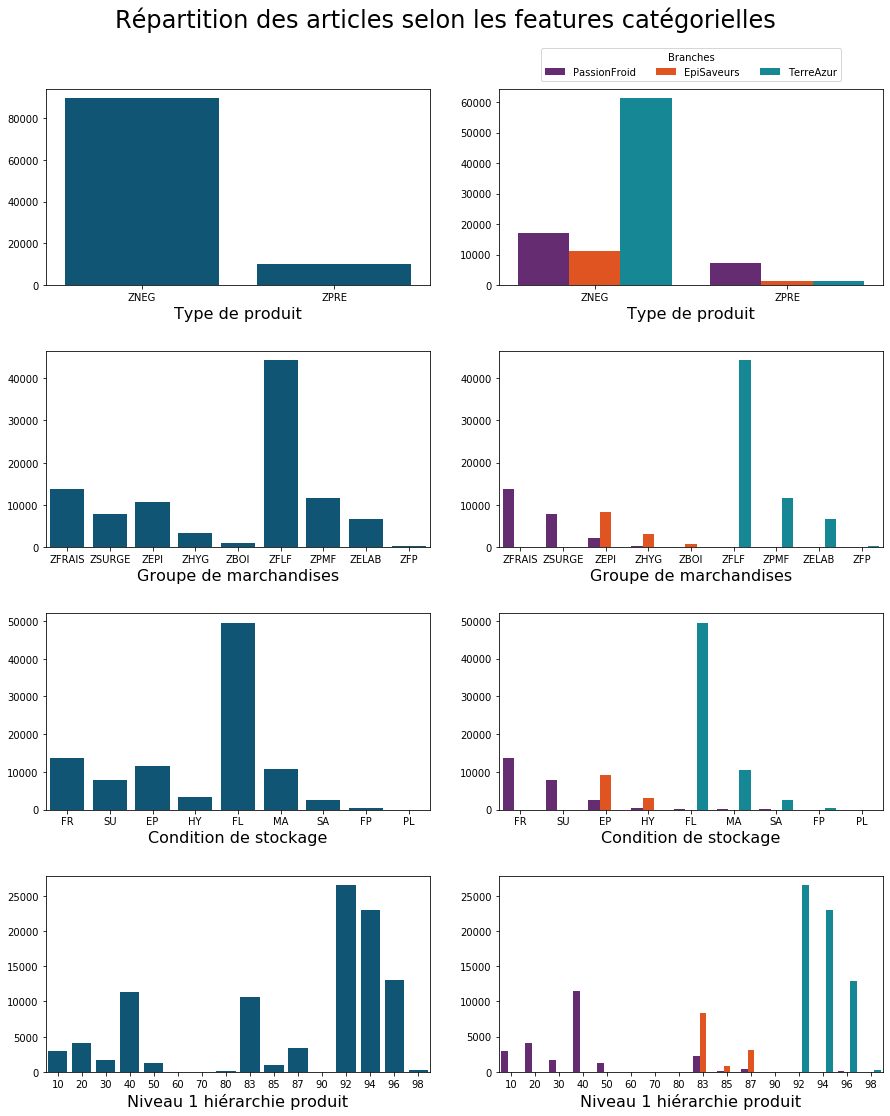
\includegraphics[width=\linewidth]{img/Repartition articles categories.png}
                \end{center}
                \caption{Répartition des articles en fonction des variable catégorielles}
                \label{fig:repart_art_categ}
            \end{figure}

            \begin{table}[htbp]
                \footnotesize
                \begin{center}
                \begin{tabular}{lccc}
\toprule
\textbf{Branche} &  PassionFroid &  EpiSaveurs &  TerreAzur \\
\textbf{Type de produit             } &               &             &            \\
\midrule
\textbf{ZNEG - Article de négoce    } &         17166 &       11048 &      61273 \\
\textbf{ZPRE - Article de prestation} &          7388 &        1193 &       1437 \\
\bottomrule
\end{tabular}

                \vspace{5pt}
                \begin{tabular}{lccc}
\toprule
\textbf{Branche} & PassionFroid & EpiSaveurs & TerreAzur \\
\textbf{Groupe de marchandises   } &              &            &           \\
\midrule
\textbf{ZSURGE - Surgelés        } &         7756 &          - &         - \\
\textbf{ZFRAIS - Frais           } &        13785 &          6 &         4 \\
\textbf{ZEPI - Epicerie          } &         2298 &       8305 &         - \\
\textbf{ZBOI - Boissons          } &          126 &        826 &         - \\
\textbf{ZHYG - Hygiène           } &          350 &       3078 &         - \\
\textbf{ZFLF - Fruits et Légumes } &            4 &          - &     44133 \\
\textbf{ZPMF - Produits de la mer} &          142 &          - &     11594 \\
\textbf{ZELAB - Produits élaborés} &           91 &          - &      6644 \\
\textbf{ZFP - Fleurs et plantes  } &            - &          - &       297 \\
\textbf{ZAUTRE - Autres          } &            2 &         26 &        38 \\
\bottomrule
\end{tabular}

                \vspace{5pt}
                \begin{tabular}{lcccc}
\toprule
\textbf{Branche} & PassionFroid & EpiSaveurs & TerreAzur &  Total \\
\textbf{Condition de stockage } &              &            &           &        \\
\midrule
\textbf{SU - Surgelés         } &         7758 &          - &         - &   7758 \\
\textbf{FR - Frais            } &        13781 &          6 &         3 &  13790 \\
\textbf{EP - Epicerie         } &         2430 &       9155 &         - &  11585 \\
\textbf{HY - Hygiène          } &          344 &       3080 &         - &   3424 \\
\textbf{FL - Fruits et légumes} &           78 &          - &     49508 &  49586 \\
\textbf{MA - Marée            } &          126 &          - &     10501 &  10627 \\
\textbf{FP - Fleurs et plantes} &            - &          - &       286 &    286 \\
\textbf{SA - Saurisserie      } &           34 &          - &      2408 &   2442 \\
\textbf{PL - Publicié         } &            2 &          - &         1 &      3 \\
\bottomrule
\end{tabular}

                \vspace{5pt}
                \begin{tabular}{lccc}
\toprule
\textbf{Branche} & PassionFroid & EpiSaveurs & TerreAzur \\
\textbf{Niveau 1 hiérarchie produit        } &              &            &           \\
\midrule
\textbf{10 - Beurre, oeufs, fromage        } &         3010 &          6 &         1 \\
\textbf{20 - Elaborés                      } &         4150 &          2 &         6 \\
\textbf{30 - Garnitures et fruits          } &         1701 &          - &         - \\
\textbf{40 - Produits carnés               } &        11413 &          - &         - \\
\textbf{50 - Produits de la mer            } &         1214 &          - &         2 \\
\textbf{60 - Consommables                  } &            1 &          - &         - \\
\textbf{70 - Emballage                     } &            - &          1 &         - \\
\textbf{80 - Publicité sur le lieu de vente} &           34 &         25 &        37 \\
\textbf{83 - Epicerie                      } &         2306 &       8296 &         - \\
\textbf{85 - Liquides                      } &          135 &        836 &         - \\
\textbf{87 - Hygiène et entretien          } &          348 &       3075 &         - \\
\textbf{90 - Services                      } &           10 &          - &         - \\
\textbf{92 - Fruits                        } &           35 &          - &     26543 \\
\textbf{94 - Légumes                       } &           37 &          - &     22929 \\
\textbf{96 - Produits de la mer Frais      } &          160 &          - &     12891 \\
\textbf{98 - Fleurs - plantes              } &            - &          - &       301 \\
\bottomrule
\end{tabular}

                \end{center}
                \caption{Utilisation des variables catégorielles article au sein des branches RHD}
                \label{tab:repart_art_categ}
                \normalsize
            \end{table}

            Possibilité d'extension: 
            - ajouter la vision produit (via les FIA)
            - faire une sorte d'heatmap qui montre la forte correlation entre les différentes variables catégorielles (et les définitions associées. Ex: ZELAB + SA = Saurisserie, etc...)

    \chapter{Les données utilisables, issues du PIM}
        \large
        Comme vu au chapitre \mref{perimetre_produit}, les données produit ne sont simplement accessibles que pour la branche \'{E}piSaveurs.
        On se focalisera donc sur cette branche pour la suite de cette étude, ainsi que sur les produits alimentaires (en excluant donc les produits d'hygiène et de chimie, cf. section \mref{produits_nonal}).
        Contrairement au chapitre précédent, ici on travaillera à la maille \emph{produit} (cf. la distinction produit vs. article section \mref{produit_article}).
        L'ensemble des tableaux et graphes de ce chapitre ont été produit via le notebook "Analyse des données du PIM", présenté en annexe \mref{code:analyse_donnees_PIM}.
        \normalsize

        \section{Données structurées}

            \subsection{Description des données structurées}

        Les données dites structurées sont l'ensemble des données qui peuvent prendre leurs valeurs dans un domaine restreint.
        Par exemple, ce sont les données booléennes, les choix issus de listes déroulantes, les valeurs numériques\dots
        Les principales données structurées pour les produits alimentaires dans le PIM sont : 
        \begin{description}
            \item[le code du produit :] calculé par le système
            \item[le fournisseur :] référence croisée vers le code du fournisseur
            \item[le type de produit :] épicerie, boisson alcoolisée, hygiène, chimie, boisson non-alcoolisée
            \item[le GTIN du produit :] identifiant numérique unique, utilisé entre autres pour l'étiquetage sous forme de code à barres~\cite{GS1_GTIN}
            \item[le type d'unité de base :] paquet, boîte, sachet, rouleau, bouteille, pot, \dots
            \item[les poids :] brut, net, net égoutté (pour les conserves)
            \item[le volume :] pour les produits liquides
            \item[les durées de vie :] le type (Date Limite de Consommation ou Date de Durabilité Minimale) et la durée (totale à fin de production, garantie à livraison)
            \item[les modes de conservation avant/après ouverture :] à température ambiante, au réfrigérateur puis à consommer sous 2 jours, \dots
            \item[les labels :] le(s) label(s) s'appliquant au produit (cf. section \ref{labels} page \pageref{labels})
            \item[les régimes particuliers :] Halal, Casher, Sans porc, Végétarien, Végétalien, \dots
            \item[les caractéristiques spéciales :] sans OGM, non traité par ionisation
            \item[la présence d'allergènes :] le niveau de présence de chacun des 14 allergènes réglementés (cf. section \mref{composition}) : absence, présence ou traces
            \item[les matières grasses utilisées :] palme, beurre, coco, tournesol, palmiste, \dots
            \item[les additifs présents :] les codes Exxx et les fonctions des additifs mis en oeuvre~\cite{additifs_regl_eu}\cite{additifs_wiki}
            \item[les données nutritionnelles obligatoires :] pour 100g ou 100mL, valeur énergétique (en kJ et kcal), matières grasses, dont acides gras saturés, Glucides, dont sucres simples, Fibres, Protéines, simplement
            \item[les données nutritionnelles facultatives :] vitamines, minéraux, omégas, \dots
            \item[les allégations nutritionnelles :] riche en, faible en, sans,\dots associé à un nutriment défini dans les 2 points précédents
            \item[le nutriscore :] note allant de A à E, définie dans la loi Santé de janvier 2016
            \item[le taux de TVA :] un des quatre taux définis dans la réglementation française
            \item[le code nomenclature douanière :] code identifiant les marchandises défini par les douanes pour la Déclaration d'\'{E}change de Biens~\cite{notions_DEB}
            \item[le pays d'origine pour la DEB :] le pays d'origine à déclarer dans la Déclaration d'\'{E}change de Biens~\cite{notions_DEB}
            \item[les informations logistiques :] il s'agit du plan de conditionnement et de palettisation du produit. Elles regroupent les différents niveaux et les quantités pour passer de l'un à l'autre (ex : 3 boites dans un cartons, 64 cartons dans une palette), les poids et dimensions de ces niveaux logistiques, leurs GTIN, \dots
        \end{description}
        
            \subsection{Analyse de ces données structurées}

                \subsubsection{Le statut des produits}
                Comme cela a été présenté à la \reffig{fig:processus_article}, le processus de gestion de l'information produit fait intervenir de multiples acteurs et peut donc être assez long.
                Un produit qui n'est pas arrivé au bout du processus et fait l'objet de contrôles et validations successives n'est pas réputé comme portant des informations correctes.
                Dans le PIM, la \og localisation \fg~du produit dans le processus est portée par son statut (c'est une simple donnée catégorielle).
                Seuls les produits au statut \og Validé \fg~sont considérés comme portant des données valides.
                La répartition des produits pour chacun des statuts est présenté à la \reffig{fig:products_status}.

                \begin{figure}[htbp]\CenterFloatBoxes
                    \begin{floatrow}
                    \ffigbox{%
                        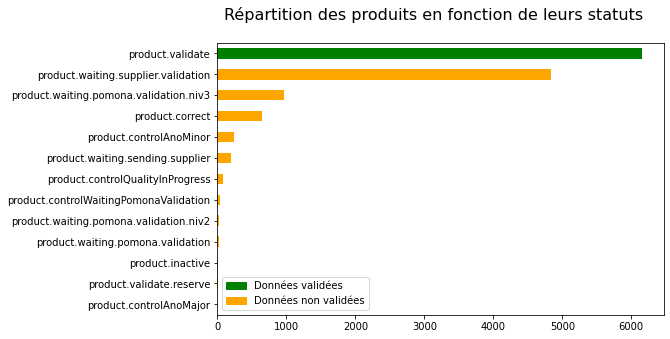
\includegraphics[width=200pt]{img/products_status.png}%
                    }{%
                      \caption{Répartition des produits par statut}%
                      \label{fig:products_status}%
                    }
                    
                    \capbtabbox[][][c]{%
                        \tiny%
                        \begin{tabular}{lc}
\toprule
{} &  state \\
\midrule
\textbf{product.validate                      } &   6240 \\
\textbf{product.waiting.supplier.validation   } &   4812 \\
\textbf{product.waiting.pomona.validation.niv3} &    906 \\
\textbf{product.correct                       } &    671 \\
\textbf{product.controlAnoMinor               } &    245 \\
\textbf{product.waiting.sending.supplier      } &    192 \\
\textbf{product.controlQualityInProgress      } &     48 \\
\textbf{product.controlWaitingPomonaValidation} &     32 \\
\textbf{product.waiting.pomona.validation.niv2} &     29 \\
\textbf{product.waiting.pomona.validation     } &     21 \\
\textbf{product.inactive                      } &     12 \\
\textbf{product.validate.reserve              } &      3 \\
\textbf{product.controlAnoMajor               } &      1 \\
\bottomrule
\end{tabular}
%
                        \normalsize%
                    }{%
                      \caption{Répartition des produits par statut}%
                    }
                    \end{floatrow}
                \end{figure}        

                De plus, comme cela a été présenté dans la section migration \mref{migration}, certains produits ont fait l'objet d'un contrôle et d'une correction après le démarrage, mais d'autres non.
                Il est nécessaire de prendre également cet aspect en compte si l'on souhaite avoir la vision des produits qui sont censés avoir des données correctes.
                La détermination du statut des produits vis-à-vis du processus de migration se fait au travers de facettes :
                \begin{itemize}
                    \item les produits qui ont été créés lors de la reprise de données initiale portent une facette "beginningMigration"
                    \item les produits créés dans le PIM après le démarrage (cas des nouveaux référencements) ne portent pas cette facette
                    \item les produits issus de la migration (portant la facette "beginningMigration") sont envoyés aux fournisseurs pour qu'ils complètent les données 
                    \item une fois que le processus de validation de l'information produit est terminé (validation des gestionnaires de référentiels), une facette "endMigration" est apposée sur le produit
                \end{itemize}
                La répartition des produits fonction de leurs statuts de migration est présenté à la \reftable{tbl:migration_status}.
                Les produits portant des données correctes, du point de vue de la migration, sont : 
                \begin{itemize}
                    \item ceux qui ont été créés après le démarrage (donc qui ont été créés avec le processus et les règles de gestion cible)
                    \item ceux qui ont été créés à la reprise, mais qui sont identifiés comme ayant terminé le processus de migration (portant la facette de fin)
                \end{itemize}

                \begin{table}[htbp]
                    \begin{center}
                    \begin{tabular}{lcc}
\toprule
{} &  Migration en cours &  Migration terminée \\
\midrule
\textbf{Créé après le démarrage} &                1657 &                   0 \\
\textbf{Créé au démarrage      } &                7212 &                4343 \\
\bottomrule
\end{tabular}

                    \caption{Répartition des produits par statut de migration}
                    \label{tbl:migration_status}
                    \end{center}
                \end{table}

                Si on combine le statut des produits avec leurs statut de migration, on peut calculer un statut \og Données valides \fg qui doit permettre d'identifier des produits avec des données de qualité.
                C'est ce statut qui sera utilisé dans les paragraphes suivants, lorsqu'on fera des anlyses relatives à la qualité des données.
                \label{def:en_qualite}
                On nommera ces statuts \og En qualité \fg et \og Hors qualité \fg pour la suite de ce document.
                La volumétrie des produits en fonction de chacun de ces statuts est présentée à la \reftable{tbl:products_quality}.

                \begin{table}[htbp]
                    \begin{center}
                    \begin{tabular}{lc}
\toprule
{} &  Répartition produit par qualité \\
\midrule
\textbf{Hors qualité} &                             8722 \\
\textbf{En qualité  } &                             4513 \\
\bottomrule
\end{tabular}

                    \caption{Répartition des produits par \og qualité des données \fg}
                    \label{tbl:products_quality}
                    \end{center}
                \end{table}

                \subsubsection{Données d'identification}
                Un exemple et une description statistique de ces données est présentées aux \reftable{tbl:exemple_idt} et \reftable{tbl:desc_idt}.
                On peut en tirer les conclusions suivantes : 
                \begin{itemize}
                    \item Les codes produits sont bien des identifiants uniques des produits : on a autant de valeurs uniques que de valeurs renseignées
                    \item Une proportion importante de produits (91\%) porte un GTIN (cf. \cite{GS1_GTIN}), ce qui reflète une \og maturité \fg des filières produits avec lesquelles travaille \'{E}piSaveurs.
                    \item Ces GTIN sont également censés être des identifiants uniques des produits. Néanmoins, comme présenté à la \reffig{fig:produit_par_GTIN}, il peut arriver que le même GTIN soit présent sur plusieurs produits. Quelques illustrations et explications sont présentées en annexe, dans le notebook d'analyse des données.
                    \item La distribution numérique des produits par fournisseur est importante. Il existe plus de 600 fournisseurs pour les 13000 produits, et l'essentiel des fournisseur n'ont qu'un nombre très limité de produits. On peut avoir une vision à la \reffig{fig:distrib_fourn_pdts} ou à la \reffig{fig:rappel_pdt_par_frn}.
                \end{itemize}

                TODO : illustrer ici les graphes suivants.

                \begin{figure}[htbp]\CenterFloatBoxes
                    \begin{floatrow}
                    \ffigbox{%
                        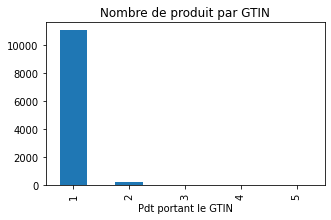
\includegraphics[width=200pt]{img/repartition_gtin.png}%
                    }{%
                      \caption{Nombre de produits par GTIN}%
                      \label{fig:produit_par_GTIN}%
                    }
                    \capbtabbox[][][c]{%
                        \begin{tabularx}{\linewidth}{lX}
\toprule
{} &  Nb de GTIN \\
\textbf{Pdt portant le GTIN} &             \\
\midrule
\textbf{1                  } &       11068 \\
\textbf{2                  } &         227 \\
\textbf{3                  } &          22 \\
\textbf{4                  } &          20 \\
\textbf{5                  } &           1 \\
\bottomrule
\end{tabularx}
%
                    }{%
                      \caption{Nombre de produits par GTIN}%
                    }
                    \end{floatrow}
                \end{figure}        

                \begin{figure}[htbp]
                    \begin{center}
                    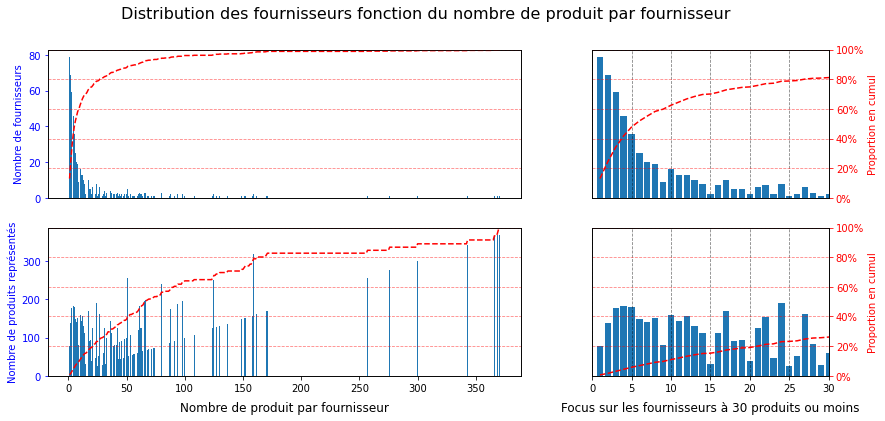
\includegraphics[width=\linewidth]{img/distribution_fournisseurs_par_prd_count.png}
                    \end{center}
                    \caption{Distribution des fournisseurs par nombre de produits}
                    \label{fig:distrib_fourn_pdts}
                \end{figure}

                \begin{figure}[htbp]
                    \begin{center}
                    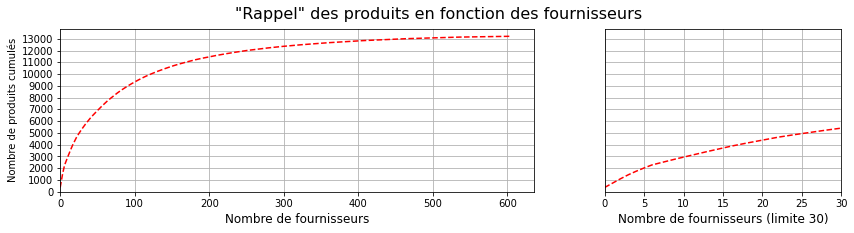
\includegraphics[width=\linewidth]{img/rappel_produit_par_fournisseur.png}
                    \end{center}
                    \caption{Le Pareto des produits en fonction des fournisseur}
                    \label{fig:rappel_pdt_par_frn}
                \end{figure}

        TODO : continuer l'analyse par domaine de données.

        
        \begin{landscape}   
            \begin{table}
                \RawFloats
                {\scriptsize
                \begin{center}
                \begin{tabular}{lcccc}
\toprule
{} &     Code produit & Code fournisseur & Type de produit &            GTIN \\
\textbf{uid                                 } &                  &                  &                 &                 \\
\midrule
\textbf{1c6a9d67-8fea-4b5e-a0c3-29f9338e1128} &  PIMP-0000004399 &  PIMF-0000000112 &  alcoholicDrink &   3080210001100 \\
\textbf{07d045b6-4cde-403d-b577-a11b899dcd29} &  PIMP-0000005503 &  PIMF-0000000060 &         grocery &   3760128846009 \\
\textbf{40b933d8-d8eb-4867-8d14-83fc999c5281} &  PIMP-0000010837 &  PIMF-0000000011 &         grocery &  13274643110097 \\
\textbf{ae72ae63-7b12-4bcf-b15e-52acff941375} &  PIMP-0000003913 &  PIMF-0000000283 &         hygiene &   3342690094301 \\
\textbf{81ed6169-03eb-44b5-a3eb-8a25e879948e} &  PIMP-0000010172 &  PIMF-0000000178 &         hygiene &            None \\
\bottomrule
\end{tabular}
%
                \caption{Exemples de codes d'identification}%
                \label{tbl:exemple_idt}%
                \bigskip\bigskip
                \begin{tabularx}{\linewidth}{lXXXX}
\toprule
{} &     Code produit & Code fournisseur & Type de produit &   GTIN \\
\midrule
\textbf{count } &            13183 &            13183 &           13183 &  12019 \\
\textbf{unique} &            13183 &              605 &               5 &  11333 \\
\textbf{top   } &  PIMP-0000011105 &  PIMF-0000000179 &         grocery &        \\
\textbf{freq  } &                1 &              370 &            8755 &    352 \\
\bottomrule
\end{tabularx}
%
                \caption{Description des codes d'identification sur le dataframe}%
                \label{tbl:desc_idt}%   
                \end{center}
                }
            \end{table}

            \begin{table}
                \RawFloats
                {\scriptsize
                \begin{center}
                \begin{tabularx}{\linewidth}{lXXXXX}
\toprule
{} & Unité de base &  Poids net &  Poids brut &  Poids net égoutté &  Volume \\
\textbf{uid                                 } &               &            &             &                    &         \\
\midrule
\textbf{4bf17478-a4fd-43b3-9920-151f73b76ba0} &           COL &      1.260 &       1.700 &                  - &       - \\
\textbf{af78f096-2406-48a4-8481-d461d6b32bb0} &           COL &      1.200 &       1.560 &                  - &       - \\
\textbf{855fcaf4-81c8-4f46-8e99-101202f07e0b} &           SAC &      1.000 &       1.040 &                  - &       - \\
\textbf{d092afe5-e0fe-42d8-ba58-dc2e9b579767} &           BTE &      0.340 &       0.360 &                  - &    0.33 \\
\textbf{995ef7a8-8d7c-4d93-9528-517ebbd60f67} &           SAC &      0.295 &       0.297 &                  - &       - \\
\bottomrule
\end{tabularx}
%
                \caption{Exemples de dimensions}%
                \label{tbl:exemple_dim}%
                \bigskip\bigskip
                \begin{tabular}{lccccc}
\toprule
{} & Unité de base &  Poids net &  Poids brut &  Poids net égoutté &    Volume \\
\midrule
\textbf{count } &         13183 &  12817.000 &   12817.000 &           1026.000 &  1911.000 \\
\textbf{unique} &            30 &          - &           - &                  - &         - \\
\textbf{top   } &           BTE &          - &           - &                  - &         - \\
\textbf{freq  } &          3051 &          - &           - &                  - &         - \\
\textbf{mean  } &             - &      3.111 &       2.985 &              1.475 &     7.751 \\
\textbf{std   } &             - &     59.623 &      42.187 &              1.133 &    78.979 \\
\textbf{min   } &             - &      0.000 &       0.000 &              0.000 &     0.000 \\
\textbf{25\%   } &             - &      0.482 &       0.535 &              0.480 &     0.500 \\
\textbf{50\%   } &             - &      1.000 &       1.100 &              1.500 &     0.900 \\
\textbf{75\%   } &             - &      3.000 &       3.291 &              2.380 &     2.500 \\
\textbf{max   } &             - &   4900.000 &    4730.500 &             10.000 &  3100.000 \\
\bottomrule
\end{tabular}
%
                \caption{Description des dimensions sur le dataframe}%
                \label{tbl:desc_dim}%  
                \end{center}
                }
            \end{table}

            \begin{table}
                \RawFloats
                {\scriptsize
                \begin{center}
                \begin{tabularx}{\linewidth}{lXXXXXXX}
\toprule
{} &  Durée de vie totale &  Durée minimale restante & Type de conservation & Conservation avant ouv. & Convervation après ouv. & Température &  data\_ok \\
\textbf{uid                                 } &                      &                          &                      &                         &                         &             &          \\
\midrule
\textbf{61908e4e-4f95-4e69-b04a-2203b5e68a84} &                 28.0 &                     18.0 &                   AM &      ambientTemperature &         coolAndDryPlace &           - &    False \\
\textbf{f254910f-8562-431e-a499-cae5e67158b7} &                540.0 &                    360.0 &                   AM &      ambientTemperature &         coolAndDryPlace &           - &     True \\
\textbf{cfbf9793-4e5f-48e7-8dc0-d7653fe47d70} &                 24.0 &                     15.0 &                   AM &         coolAndDryPlace &         coolAndDryPlace &           - &    False \\
\textbf{e165da13-1f8b-4a2f-9271-fc507e571cbb} &                    - &                        - &                   AM &                       - &                       - &           - &    False \\
\textbf{8c764293-ba0a-4103-8465-23a4f5eff7bb} &                360.0 &                    240.0 &                   AM &      ambientTemperature &            notConcerned &           - &    False \\
\bottomrule
\end{tabularx}
%
                \caption{Exemples de conservation}%
                \label{tbl:exemple_cons}%
                \bigskip\bigskip
                \begin{tabularx}{\linewidth}{lXXXXXX}
\toprule
{} &  Durée de vie totale &  Durée minimale restante & Type de conservation & Conservation avant ouv. & Convervation après ouv. & Température \\
\midrule
\textbf{count } &             8946.000 &                 9466.000 &                12806 &                    9977 &                    9947 &          21 \\
\textbf{unique} &                    - &                        - &                    2 &                       7 &                      18 &           9 \\
\textbf{top   } &                    - &                        - &                   AM &      ambientTemperature &         coolAndDryPlace &          15 \\
\textbf{freq  } &                    - &                        - &                12772 &                    8270 &                    4512 &           6 \\
\textbf{mean  } &              651.406 &                  351.618 &                    - &                       - &                       - &           - \\
\textbf{std   } &              487.412 &                  380.255 &                    - &                       - &                       - &           - \\
\textbf{min   } &                0.000 &                    0.000 &                    - &                       - &                       - &           - \\
\textbf{25\%   } &              360.000 &                  180.000 &                    - &                       - &                       - &           - \\
\textbf{50\%   } &              540.000 &                  300.000 &                    - &                       - &                       - &           - \\
\textbf{75\%   } &              900.000 &                  480.000 &                    - &                       - &                       - &           - \\
\textbf{max   } &             9999.000 &                 9999.000 &                    - &                       - &                       - &           - \\
\bottomrule
\end{tabularx}
%
                \caption{Description des conservations sur le dataframe}%
                \label{tbl:desc_cons}%  
                \end{center}
                }
            \end{table}

        \normalsize
        \end{landscape}

        \section{Données non structurées}
        
            \subsection{Les libellés}

            Plusieurs libellés permettent de faire référence à chaque produit, avec des usages distincts:
            \begin{description}
                \item[Libellé temporaire unité de besoin :] il s'agit simplement d'un libellé qui est choisi par la personne à l'origine de la demande de référencement produit (souvent l'acheteur, cf. \reffig{fig:processus_article}), afin que le fournisseur comprenne sur quel produit porte le référencement.
                \item[Désignation du produit fournisseur :] c'est le libellé qui est donné par le fournisseur afin d'identifier simplement son produit.
                \item[Code article interne fournisseur :] c'est l'identifiant du produit, dans le système de gestion du fournisseur. Il s'agit généralement de codes, avec autant de formats distincts que de fournisseur venant contribuer.
                \item[Marque commerciale du produit :] il s'agit du nom de la marque commerciale du produit. 
                \item[Dénomination réglementaire :] c'est le libellé qui doit décrire de manière neutre le produit, sans notion liée au marketing (telle que la marque, entre autres), et qui doit obligatoirement figurer sur l'emballage du produit.
                \end{description}

            Des exemples de libellés sont présentés à la \reftable{tbl:exemple_lib}.

            {\renewcommand{\arraystretch}{2}%
            \begin{table}[htbp]
                {\scriptsize
                \begin{center}%
                \begin{tabular}{p{4cm}p{4cm}p{2cm}p{2cm}p{3cm}}
\toprule
                      Libellé temporaire &          Désignation produit fournisseur & Code interne fournisseur & Marque commerciale &            Dénomination réglementaire \\
\midrule
      VIN BEAUJO NOUVEAU(75CLX6) D MOREL &                       BEAUJOLAIS NOUVEAU &                  BN 2019 &    DOMINIQUE MOREL &                              VIN  AOP \\
     COCKTAIL FRT NATUREL BTE 5/1X3 DUNE &  COCKTAIL DE FRUITS A L'EAU - FORMAT 5/1 &                COC5EODUR &  DUNE Restauration &            COCKTAIL DE FRUITS A L'EAU \\
    Sauce barbecue en coupelle 20 g GYMA &     Sauce barbecue en coupelle 20 g GYMA &                   400937 &               GYMA &                        Sauce Barbecue \\
 Confiture abricot en bocal 450 g VALADE &  Confiture abricot en bocal 450 g VALADE &                 PF100006 &  VALADE EN CORREZE &                  Confiture d'abricots \\
 Confiture extra de figue en bocal verre &  BONNE MAMAN CONF FIGUES VIOLETTE    370 &                 20000929 &        BONNE MAMAN &  Confiture Extra de Figues violettes. \\
\bottomrule
\end{tabular}
%
                \caption{Exemples de libellés produit}%
                \label{tbl:exemple_lib}%
                \end{center}%
                }
            \end{table}
            }

            \subsection{Les listes d'ingrédients}
            \label{listes_ingredients}

            L'autre grand type de donnée non structurées sont les listes d'ingrédients.
            La construction des listes d'ingrédients doit suivre les règles suivantes, même si l'application n'est pas toujours parfaitement respectée :
            \begin{itemize}
                \item elle doit détailler l'ensemble des ingrédients, y compris les additifs et les arômes
                \item elle doit être triée par ordre d'importance pondérale décroissante (i.e. les ingrédients les plus représentatifs en poids doivent être cités en premier)
                \item la quantité de certains ingrédients (en pourcentage de la masse) par exemple ceux mis en valeur sur l'étiquetage ou dans la dénomination de vente (ex. gâteau aux fraises, pizza au jambon)
            \end{itemize}
            Même s'il ne s'agit pas d'une exigence réglementaire, le Groupe Pomona demande à ses fournisseurs de ne pas distinguer les ingrédients par phase comme cela se fait parfois.
            Cela signifie, par exemple, séparer une partie de la composition du produit (la pâte de la garniture pour une tarte, la sauce et les raviolis, \dots).
            De telles pratiques peuvent parfois induire le consommateur en erreur, comme par exemple dans la liste d'ingrédients suivante (s'applique à des chips de légumes):
            \begin{quotation}
                Légumes 64\% (betterave, panais, carottes, patates douces), huile de tournesol, sel marin.
            \end{quotation}
            Sans l'artifice d'avoir regroupé les légumes en une seule phase, le premier ingrédient de la liste aurait pu être l'huile de tournesol, qui est un ingrédient moins attractif pour un consommateur de chips de légumes.

            Quelques exemples de listes d'ingrédients sont présentées à la \reftable{tbl:exemple_ingred}.

            {\renewcommand{\arraystretch}{2}%
            \begin{table}[htbp]
                {\scriptsize
                \begin{center}%
                \begin{tabular}{p{5cm}l}
\toprule
                                        Désignation produit fournisseur &                                                                                                                                                                                              Liste d'ingrédients \\
\midrule
                                            HARICOTS BLANCS À LA TOMATE &                                                                                                                        Haricots blancs (UE et non UE), eau, sel, tomate concentré, antioxydant : acide citrique. \\
                                                 POIVRE VERT DÉSHYDRATÉ &                                                                                                                                                                                                 100\% poivre vert \\
            Crème de marron de l'Ardèche en boîte 500 g CLEMENT FAUGIER &                                                                                                                        Châtaignes 50\%, sucre, marrons glacés, sirop de glucose, eau, extrait naturel de vanille  \\
 Velouté de poireaux pommes de terre hyposodé en sachet 800 g NEFF MADA &  Pomme de terre 32 \%, amidon modifié de pomme de terre, fécule de pomme de terre, maltodextrine de blé, poireau 8 \%, arômes naturels, sucre, oignon, antiagglomérant : E551 "nano", plantes aromatiques, curcuma \\
                         Poivre Kampot rouge en pot 50 g TERRE EXOTIQUE &                                                                                                                                                                                      Poivre de Kampot rouge 100\% \\
\bottomrule
\end{tabular}
%
                \caption{Exemples de listes d'ingrédients}%
                \label{tbl:exemple_ingred}%
                \end{center}%
                }
            \end{table}
            }

            \emphbox{
            Les contraintes ci-dessus s'appliquant aux listes d'ingrédients font qu'en général, il s'agit d'une énumération d'ingrédients, sans doublon.
            }


        \section{Pièces jointes}
            \label{pieces_jointes}

            Dans le PIM, les pièces jointes - intéressantes au titre de l'information produit - gérées au niveau du produit sont les suivantes :
            \begin{itemize}
                \item les fiches techniques fournisseur
                \item les étiquettes produits
            \end{itemize}
    
            D'autres types de pièces jointes sont gérées, mais elle ne seront pas décrites dans le détail (car non pertinente pour le cas d'usage présenté):
            \begin{description}
                \item[les certificats des labels : ] ce sont des documents pdf produits par les organismes de certification attestant qu'un produit peut porter un label. Ils sont mis à disposition par les fournisseurs
                \item[les images produit : ] ce sont des visuels des produits (photographies ou images construites) qui visent à être utilisées dans des catalogues ou sur les sites de vente en ligne
                \item[les fiches logistiques : ] ce sont des fichiers qui viennent compléter les informations de la fiche technique lorsque cette dernière ne porte pas les informations relatives à la hiérarchie logistique. 
                \item[les fiches techniques et argumentaires Pomona : ] ce sont des documents pdf produits par le PIM, stockées sur les articles, qui reprennent des informations produit et article (cf. section \mref{produit_article}). Elles sont transmises aux clients ou utilisés par les commerciaux Pomona.
                Elles permettent d'avoir une présentation uniforme de l'ensemble de l'assortiment (les fiches techniques fournisseur ont des formats très variables)
            \end{description}

            \subsection{Fiches techniques fournisseur}
            \label{fiches_techniques}

                \subsubsection{Généralités sur les fiches techniques}
            Une fiche technique fournisseur est un document, d'une à une dizaine de pages, qui reprend l'essentiel des informations techniques à propos du produit.
            Elles portent globalement l'ensemble des informations produit telles que présentées à la section \mref{info_produit}.
            C'est le document le plus complet vis-à-vis des informations produit, il porte en général des informations complémentaires à toutes les informations présentes sur l'emballage du produit (les étiquettes).
            En général, une fiche technique ne porte d'information que pour un unique produit, mais dans le cas d'assortiments, les informations peuvent être relatives à plusieurs d'entre eux. Cf. la fiche technique pour l'assortiment de confitures, présentée en annexe \mref{ex:FT_confiture}.
            Les fiches techniques fournisseur sont des pièces jointes qui sont collectées par la branche \'{E}piSaveurs depuis la mise en place du logiciel de gestion historique GIP (cf. section \mref{GIP}), et il s'agit d'une données obligatoire dans le PIM également.
            
                \subsubsection{Le format des fiches techniques}
            Dans le PIM, ces pièces jointes sont collectées et stockées sous forme de pdf (les autres formats de fichier ne sont pas autorisés).
            Sauf de rares exceptions, il s'agit de fichiers issus de logiciels de traitement de texte, au format A4 portrait.
            Ce sont des documents techniques, et sont donc en général très structurés, avec des paragraphes, sous-paragraphes, tableaux, \dots
            Comme cela se constate aisément sur les exemples présentés en annexe, même si les informations portées sont sensiblement toujours les mêmes, les formats de ces documents sont extrêmement variables.
            Il n'y a aucun standard réglementaire ou normatif relatif à la construction de ces fiches, chaque industriel constitue donc son propre format.
            On a donc un foisonnement de formats différents.

                \subsubsection{Focus sur le mode de présentation de quelques informations}
            Les informations produits sont en général présentées de la manière suivantes dans les fiches techniques :
            \begin{description}
                \item[Liste d'ingrédients : ] elle est quasiment toujours présentée sous forme de texte (identique à la liste d'ingrédients telle qu'affichée sur l'emballage du produit), mais elle peut également être présentée sous forme de tableau. Cf. la fiche technique présentée en annexe \mref{ex:FT_poivron} (celle-ci ne porte pas de liste d'ingrédients sous forme de texte)
                \item[Allergènes : ] il peuvent être :
                \begin{itemize}
                    \item soit mis en évidence dans la liste d'ingrédients via la police (gras, souligné, majuscules)
                    \item soit listés hors de la liste d'ingrédient, sous forme de texte. Cf. la fiche technique présentée en annexe \mref{ex:FT_pannacotta}
                    \item soit listés sous forme d'un tableau reprenant l'ensemble des allergènes réglementaires, et le niveau de présence associé (présence, contamination croisée ou absence). Cf. la fiche technique présentée en annexe \mref{ex:FT_ciboulette}
                \end{itemize}
                \item[Données nutritionnelles : ] les données nutritionnelles sont en général présentées sous forme de tableau dans les fiches techniques. De plus, les informations nutritionnelles sont souvent données pour 100 grammes (ou 100 millilitres), ce qui est réglementaire, mais également parfois pour une portion. La taille de la portion est définie arbitrairement par le fournisseur.
                Cf. la fiche technique de la préparation pour panna cotta \mref{ex:FT_pannacotta}.
                \item[Données logistiques : ] les informations relatives à la hiérarchie logistiques se présentent souvent sous forme de tableaux.
                L'interprétation de ces tableaux est généralement complexe et nécessite un peu de réflexion.
            \end{description}
            
            \subsection{\'{E}tiquettes produit}
            \label{etiquettes_produit}

            \subsubsection{Généralités sur les étiquettes}
            L'étiquette produit est la partie de l'emballage du produit qui porte les informations produit.
            Selon la technologie de l'emballage - très liée au fait que le produit est plutôt brut ou plutôt transformé - il peut s'agir :
            \begin{itemize}
                \item d'une photo de l'étiquette collante apposée sur l'extérieur de l'emballage du produit (cf. exemple des étiquettes de lentilles \mref{ex:ET_lentilles} ou de sauce soja \mref{ex:ET_saucesoja})
                \item d'un applat de l'emballage, ou son bon-à-tirer, qui est le document qui est ensuite envoyé aux chaînes de production pour impression (cf. exemple du bon à tirer pour la préparation pour panna cotta \mref{ex:ET_pannacotta})
                \item ou de tout autre visuel montrant une partie indissociable de l'emballage physique du produit (ex : un photo de la face de l'emballage qui porte les inforations produit, cf. l'étiquette des madeleines \mref{ex:ET_madeleine})
            \end{itemize}
            Pour résumer, l'étiquette est une pièce jointe qui représente l'information produit qui \og voyage avec le produit \fg.
            La cohérence entre les données de l'étiquette et l'information produit transmises aux client est un enjeu majeur, dans la mesure où ce sont en général les informations portées par le produit physique qui sont correctes.
            La collecte systématique des étiquettes produit est une nouveauté arrivée avec la mise en place du PIM pour \'{E}piSaveurs (mai 2019).
            En théorie, les étiquettes mises à disposition par les fournisseurs devraient systématiquement porter les informations réglementaires.
            Or, du fait de la relative nouveauté de cette collecte, les pièces jointes transmises ne sont pas toujours conformes (cf. l'étiquette des lentilles \mref{ex:ET_lentilles}, qui ne portent aucune information nutritionnelle ou de composition).

            \subsubsection{Le format des étiquettes}
            Comme les fiches techniques, ces pièces jointes sont collectées et stockées sous forme de pdf (les autres formats de fichier ne sont pas autorisés).
            Du fait que les natures mêmes de ces pièces jointes sont diverses (cf. paragraphe précédent), il n'existe pas de format prédominant.

            \subsubsection{Focus sur le mode de présentation de quelques informations}
            Les étiquettes portent moins d'information que les fiches techniques.
            Par exemple, elles ne portent pas d'information sur la hiérarchie logistique, les données administratives (tel que le taux de TVA ou la nomenclature douanière), les codes d'identification (hormis le GTIN qui est présent sur le code à barre), \dots
            Les durées de vie ne sont pas mentionnées : sur l'emballage d'un produit seule la date limite apparaît, et elle dépend du lot de production.
            En règle générale, hormis quelques allégations volontairement affichées par l'industriel, l'étiquette ne porte que les informations réglementaires.
            Les information produit positionnées sur l'étiquette se présentes de la manière suivante :
            \begin{description}
                \item[Liste d'ingrédients : ] elle est toujours présentée sous forme d'un texte énumérant les ingrédients (cf. la section \mref{listes_ingredients} qui détaille le contenu d'une liste d'ingrédients)
                \item[Allergènes : ] ils sont uniquement mis en évidence dans la liste d'ingrédients, par l'utilisation d'une police spécifique (gras, souligné, majuscule, \dots). Cela peut se constater par exemple sur l'étiquette de madeleines \mref{ex:ET_madeleine} ou celle de la sauce soja \mref{ex:ET_saucesoja}
                \item[Données nutritionnelles : ] les données nutritionnelles se présentent souvent sous forme d'un tableau, toujours avec les valeurs pour 100 grammes ou 100 millilitres, et parfois pour une portion.
                Il peut arriver, plutôt pour les produits peu transformés, que ces données soient simplement écrite sous forme de texte tel que \begin{quote}\'{E}nergie : 1101 kJ/260 kcal, Glucides : 57 g, Sucres : 52 g, Protéines : 4,3 g, Sel : 7,1 g\end{quote} 
            \end{description}           

        \section{Récapitulatif de la complétude des données}

        Mettre ici un ou plusieurs tableaux récapitulatifs illustrant les données possédées quantitativement.

        Montrer également la complétude en fonction du statut, de la date de création, et des facettes de migration.

        Mettre l'exemple du champ "acide gras trans >1\%"

        \section{Analyse qualitative des données}
        
            \subsection{\'{E}valuation de la qualité des données}
        Montrer qu'un sondage basique fait que la qualité actuelle est perfectible


            \subsection{Types de pdf possédés}
        Dire ici qu'il y a finalement beaucoup de pdf qui possèdent des textes extractibles vs. uniquement des images.

        \section{Les données \og manuellement étiquetées \fg}
        \label{manually_labelled_data}

            \subsection{Pour répondre à quel besoin ?}

            La qualité des données actuellement présentes dans le système fait que la cohérence entre les listes d'ingrédients du PIM et celles présentes dans les fiches techniques n'est pas assurée.
            Comme dans tout modèle de machine learning se basant sur des données, il est indispensable ici d'avoir des données dont on est sûrs de la qualité.
            Il a donc été décidé d'étiqueter manuellement un échantillon représentatif de fiches techniques, en leur faisant correspondre leurs listes d'ingrédients.

            \subsection{Mode de constitution de l'échantillon}
            
            Le code pour la constitution de l'échantillon est présenté dans le notebook en annexe \mref{code:ground_truth}.

            Les règles de gestion adoptées pour la constitution de cet échantillon sont les suivantes :
            \begin{itemize}
                \item On constitue un échantillon de 500 fiches techniques étiquetées
                \item On se limite aux produits d'\'{E}picerie et de Boisson non alcoolisée, car ce sont les produits pour lesquels la réglementation impose d'afficher une liste d'ingrédients aux consommateurs
                \item On stratifie cet échantillon par type de produit (\'{E}picerie vs. Boisson non alcoolisée)
                \item On se limite évidemment à des produits qui possèdent une fiche technique
            \end{itemize}
            Il aurait pu être intéressant de se limiter aux produits \og en qualité \fg (cf. les définitions données à la section \mref{def:en_qualite} sur les statuts des produits), mais l'étiquetage manuel avait été fait avant l'analyse de ces statuts.
            La constitution de cet échantillon s'est traduite par la génération d'un fichier csv de 500 lignes, avec 3 colonnes : 
            \begin{itemize}
                \item l'uid du produit de l'échantillon
                \item la désignation produit fournisseur
                \item une colonne vide, visant à accueillir les listes d'ingrédients lors de l'étiquetage manuel
            \end{itemize}

            \subsection{Méthodologie de l'étiquetage manuel}

            Cette activité s'est faite simplement, dans un environnement Windows : 
            \begin{itemize}
                \item les pièces jointes ont été téléchargées localement, dans des dossiers portant l'uid du produit associé
                \item le csv contenant les uid et les désignation produit fournisseur a été ouvert dans le tableur Microsoft Excel
                \item en prenant chaque uid séquentiellement, il était relativement rapide de rechercher localement la fiche technique correspondante dans l'explorateur de fichier et de l'ouvrir
                \item le plus souvent, il était possible de copier/coller la liste d'ingrédient dans le tableur Excel
                \item le fichier a ensuite été à nouveau sauvegardé au format csv, afin de pouvoir être chargé dans pandas
            \end{itemize}

            \subsection{Règles de gestion pour l'étiquetage manuel}
        
            Expliquer que l'exercice n'est pas simple (car pas mal de petites spécificités sur les contenus). 
            Parler des produits bruts, pour lesquels on n'a parfois pas de liste d'ingrédients.
            + la filière boissons qui est moins structurée.
            Expliciter les règles de gestion qui ont été listées pendant l'étiquetage manuel

            \subsection{Confrontation avec le contenu du PIM}
            Evaluer la cohérence entre étiquettes manuelles et contenu du PIM
